% Options for packages loaded elsewhere
% Options for packages loaded elsewhere
\PassOptionsToPackage{unicode}{hyperref}
\PassOptionsToPackage{hyphens}{url}
\PassOptionsToPackage{dvipsnames,svgnames,x11names}{xcolor}
%
\documentclass[
  10pt,
  letterpaper,
  DIV=11,
  numbers=noendperiod]{scrartcl}
\usepackage{xcolor}
\usepackage{amsmath,amssymb}
\setcounter{secnumdepth}{5}
\usepackage{iftex}
\ifPDFTeX
  \usepackage[T1]{fontenc}
  \usepackage[utf8]{inputenc}
  \usepackage{textcomp} % provide euro and other symbols
\else % if luatex or xetex
  \usepackage{unicode-math} % this also loads fontspec
  \defaultfontfeatures{Scale=MatchLowercase}
  \defaultfontfeatures[\rmfamily]{Ligatures=TeX,Scale=1}
\fi
\usepackage{lmodern}
\ifPDFTeX\else
  % xetex/luatex font selection
\fi
% Use upquote if available, for straight quotes in verbatim environments
\IfFileExists{upquote.sty}{\usepackage{upquote}}{}
\IfFileExists{microtype.sty}{% use microtype if available
  \usepackage[]{microtype}
  \UseMicrotypeSet[protrusion]{basicmath} % disable protrusion for tt fonts
}{}
% Make \paragraph and \subparagraph free-standing
\makeatletter
\ifx\paragraph\undefined\else
  \let\oldparagraph\paragraph
  \renewcommand{\paragraph}{
    \@ifstar
      \xxxParagraphStar
      \xxxParagraphNoStar
  }
  \newcommand{\xxxParagraphStar}[1]{\oldparagraph*{#1}\mbox{}}
  \newcommand{\xxxParagraphNoStar}[1]{\oldparagraph{#1}\mbox{}}
\fi
\ifx\subparagraph\undefined\else
  \let\oldsubparagraph\subparagraph
  \renewcommand{\subparagraph}{
    \@ifstar
      \xxxSubParagraphStar
      \xxxSubParagraphNoStar
  }
  \newcommand{\xxxSubParagraphStar}[1]{\oldsubparagraph*{#1}\mbox{}}
  \newcommand{\xxxSubParagraphNoStar}[1]{\oldsubparagraph{#1}\mbox{}}
\fi
\makeatother


\usepackage{longtable,booktabs,array}
\usepackage{calc} % for calculating minipage widths
% Correct order of tables after \paragraph or \subparagraph
\usepackage{etoolbox}
\makeatletter
\patchcmd\longtable{\par}{\if@noskipsec\mbox{}\fi\par}{}{}
\makeatother
% Allow footnotes in longtable head/foot
\IfFileExists{footnotehyper.sty}{\usepackage{footnotehyper}}{\usepackage{footnote}}
\makesavenoteenv{longtable}
\usepackage{graphicx}
\makeatletter
\newsavebox\pandoc@box
\newcommand*\pandocbounded[1]{% scales image to fit in text height/width
  \sbox\pandoc@box{#1}%
  \Gscale@div\@tempa{\textheight}{\dimexpr\ht\pandoc@box+\dp\pandoc@box\relax}%
  \Gscale@div\@tempb{\linewidth}{\wd\pandoc@box}%
  \ifdim\@tempb\p@<\@tempa\p@\let\@tempa\@tempb\fi% select the smaller of both
  \ifdim\@tempa\p@<\p@\scalebox{\@tempa}{\usebox\pandoc@box}%
  \else\usebox{\pandoc@box}%
  \fi%
}
% Set default figure placement to htbp
\def\fps@figure{htbp}
\makeatother





\setlength{\emergencystretch}{3em} % prevent overfull lines

\providecommand{\tightlist}{%
  \setlength{\itemsep}{0pt}\setlength{\parskip}{0pt}}



 


\usepackage{xcolor, soul}
\definecolor{Light}{gray}{.90}
\sethlcolor{Light}
\let\OldTexttt\texttt
\renewcommand{\texttt}[1]{\OldTexttt{\hl{#1}}}
\usepackage{caption}
\captionsetup{font=small, labelfont=bf}
\setlength{\parindent}{0pt}
\setlength{\parskip}{1.25ex}
\KOMAoption{captions}{tableheading}
\makeatletter
\@ifpackageloaded{caption}{}{\usepackage{caption}}
\AtBeginDocument{%
\ifdefined\contentsname
  \renewcommand*\contentsname{Table of contents}
\else
  \newcommand\contentsname{Table of contents}
\fi
\ifdefined\listfigurename
  \renewcommand*\listfigurename{List of Figures}
\else
  \newcommand\listfigurename{List of Figures}
\fi
\ifdefined\listtablename
  \renewcommand*\listtablename{List of Tables}
\else
  \newcommand\listtablename{List of Tables}
\fi
\ifdefined\figurename
  \renewcommand*\figurename{Figure}
\else
  \newcommand\figurename{Figure}
\fi
\ifdefined\tablename
  \renewcommand*\tablename{Table}
\else
  \newcommand\tablename{Table}
\fi
}
\@ifpackageloaded{float}{}{\usepackage{float}}
\floatstyle{ruled}
\@ifundefined{c@chapter}{\newfloat{codelisting}{h}{lop}}{\newfloat{codelisting}{h}{lop}[chapter]}
\floatname{codelisting}{Listing}
\newcommand*\listoflistings{\listof{codelisting}{List of Listings}}
\makeatother
\makeatletter
\makeatother
\makeatletter
\@ifpackageloaded{caption}{}{\usepackage{caption}}
\@ifpackageloaded{subcaption}{}{\usepackage{subcaption}}
\makeatother
\usepackage{bookmark}
\IfFileExists{xurl.sty}{\usepackage{xurl}}{} % add URL line breaks if available
\urlstyle{same}
\hypersetup{
  pdftitle={Pairwise between-family d' calculations},
  pdfauthor={Al Xin},
  colorlinks=true,
  linkcolor={blue},
  filecolor={Maroon},
  citecolor={Blue},
  urlcolor={Blue},
  pdfcreator={LaTeX via pandoc}}


\title{Pairwise between-family d' calculations}
\author{\small Al Xin}
\date{Jul 17, 2026}
\begin{document}
\maketitle


\section{Data}\label{data}

\subsection{Loading}\label{loading}

See \texttt{20260625.qmd} for reference. For now, analysis will be
limited to reliable sites and images with naturalistic structure.

\section{LDA}\label{lda}

\subsection{Procedure}\label{procedure}

Lee et al.~trained the population decoder by:

\begin{enumerate}
\def\labelenumi{\arabic{enumi}.}
\tightlist
\item
  Taking a training set of repetitions (15-fold CV separated by sample)
  (\textbf{this notebook}).
\item
  Projecting the population response to non-blank images onto the first
  several principal components. Gerick mentioned this step was omitted
  in later analyses. Performing LDA on the original data works fine and
  removes the issue of finding PCs for combinations of subjects.
\item
  Applying linear discriminant analysis (LDA) to find the axis
  separating the naturalistic and noisy textures. For between-family
  discrimination, this is replaced by finding the axis best separating
  the families.
\item
  Projecting held-out responses on the axis, then reporting the \(d'\)
  on the resulting one-dimensional values.
\end{enumerate}

\subsection{Variations}\label{variations}

Due to the low number of repetitions per individual image (6
repetitions), it is probably untenable to train LDA on pairwise sample
comparisons. For low repetition analyses, I'll apply random dichotomies
to increase the power.

LDA can be applied on:

\begin{enumerate}
\def\labelenumi{\arabic{enumi}.}
\tightlist
\item
  Pairwise family comparisons with 15-fold CV (holdout is one of the
  sample IDs)
\item
  Random dichotomies within families with 6-fold CV (holdout is one of
  the repetition IDs)
\item
  Random dichotomies between families with 6-fold CV (similar to the
  previous variation but with samples taken from different families)
\end{enumerate}

\subsection{Procedure for this
notebook}\label{procedure-for-this-notebook}

I subsampled 30 sites for each region out of the reliable sites.
Subsampling did not consider simultaneous recording, so the subsampled
sites may include more than one array. I fit LDA with
\texttt{MASS::lda()} and found the projections with the \texttt{x}
output of \texttt{predict.lda()} on the test set.

\section{Pairwise between-family
distances}\label{pairwise-between-family-distances}

For each family pair, data is saved as a list with:

\begin{itemize}
\tightlist
\item
  \texttt{dprimes}: a data frame

  \begin{itemize}
  \tightlist
  \item
    \texttt{mu}: the difference in means
  \item
    \texttt{sd}: the combined standard deviation
  \item
    \texttt{data\_split}: the \texttt{trn} or \texttt{tst} reading
  \item
    \texttt{dprime}: the calculated Cohon's \(d'\), found as \texttt{mu}
    / \texttt{sd}
  \item
    \texttt{k}: the label for the fold in 15-fold CV (corresponding to
    15 samples)
  \end{itemize}
\item
  \texttt{scalings}: a numeric \(15 \times 73\) matrix corresponding to
  15 samples by the number of sites (here, determined by the number of
  reliable sites)
\item
  \texttt{group\_ids}: a numeric vector containing the group IDs
  included in the pair
\end{itemize}

Within this notebook, I mostly sanity tested some of the procedures. See
\texttt{scripts/pairwise\_family.R} for the code. I ran the calculations
in the Stats server.

\(d'\) values are reported as the average across the 15 folds. See
Figure~\ref{fig-dprime} for histograms of the pairwise comparison \(d'\)
values (subsampled for 30 sites), separated by region. The trend in the
results seem consistent with Gerick's poster (copied in
Figure~\ref{fig-areadne2024} for reference), with the center of the
histogram generally tending toward higher \(d'\) with higher visual
regions with the trend reversing in IT. Both the difference in means and
combined SD tend to increase with higher visual regions, again with the
trend reversing in IT. This may indicate that for V1 to V2 to V4, the
firing patterns tend to be more spread out, with the increased variance
compensated by better separation of the groups. There does not seem to
be a notable difference in train and test \(d'\)
(Figure~\ref{fig-dprime}, right).

Though the relative differences in \(d'\) distributions seem similar to
Gerick's previous results, the scales are inconsistent, with Gerick
finding \(d'\) values as high as around 6 for V4 (my max: 1.3).
Possibly, he calculated LDA on averages over repetitions, thus lowering
the combined SD (the denominator of the \(d'\)). It may also be due to
differences in the number of sampled sites.

\begin{figure}

\centering{

\pandocbounded{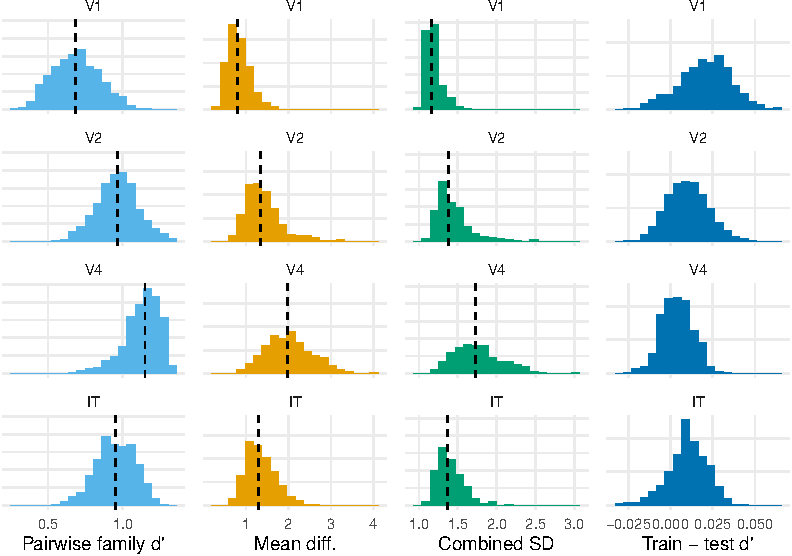
\includegraphics[keepaspectratio]{20260715_files/figure-pdf/fig-dprime-1.pdf}}

}

\caption{\label{fig-dprime}Histogram of d', mean differences, combined
SD, and train-test difference for each pairwise family comparison,
separated by region. Vertical line indicates the median.}

\end{figure}%

\begin{figure}

\centering{

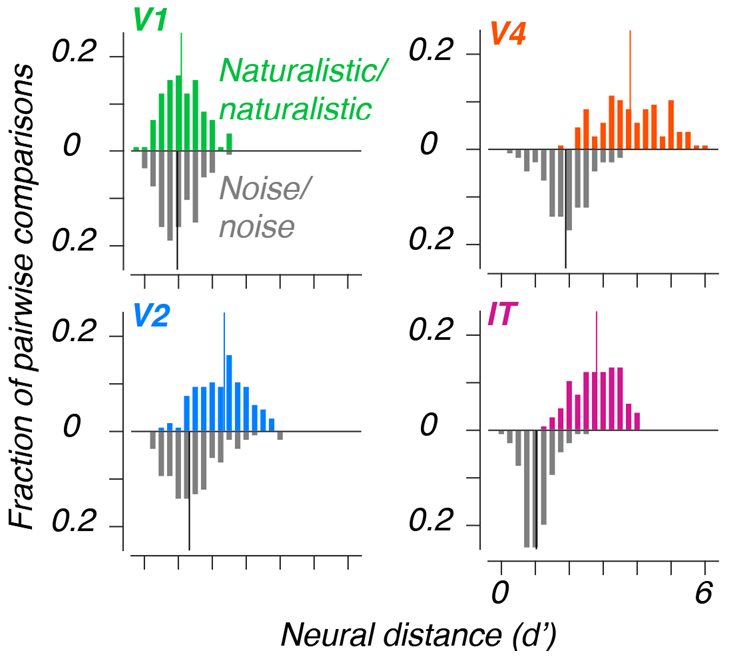
\includegraphics[width=0.4\linewidth,height=\textheight,keepaspectratio]{../../reports/img/lee2024-poster-1.png}

}

\caption{\label{fig-areadne2024}Histograms of pairwise comparisons, for
naturalistic-naturalistic comparisons (colored bars), and noise-noise
comparisons (gray). Lines depict medians. The figure was originally
vertical but I rearranged it, so the axes are consistent for all
quadrants.}

\end{figure}%




\end{document}
